\documentclass{beamer}
\usepackage[utf8]{inputenc}
\usepackage{graphicx}
\graphicspath{ {./images/} }

\title{Vývoj samoříditelné platformy}
\author{Filip Peterek}
\institute{Vysoká škola Báňská - Technická univerzita Ostrava}
\date{Květen 2021}

\AtBeginSection[]{
    \begin{frame}
        \frametitle{Obsah}
        \tableofcontents[currentsection]
    \end{frame}
}

\begin{document}

\frame{\titlepage}

\section{Cíl práce}
\begin{frame}
    \frametitle{Cíl práce}

    \begin{itemize}
        \item Prozkoumat možnosti autonomního řízení vozidla
        \item Implementovat autonomní řízení v kampusu VŠB-TUO
        \item Implementovat komunikaci s vozidlem pomocí rozhraní CAN
        \item Implementovat simulátor vozidla sloužící k testování SW
    \end{itemize}

\end{frame}

\section{Výstup práce}
\begin{frame}
    \frametitle{Výstup práce}
    
    \begin{itemize}
        \item Následování grafických kódů
        \item Problematické řízení pomocí GPS souřadnic
        \item Rozpracované řízení využívající vstupů z kamer, LiDARu i GPS
        \item Webová aplikace sloužící k ovládání vozidla
        \item Python skript sloužící ke stahování a exportu mapových podkladů
        \item Simulátor vozidla
        \item Komunikace s vozidlem za využití rozhraní CAN
        \item Android aplikace logující GPS souřadnice
    \end{itemize}
\end{frame}

\section{Architektura projektu}

\begin{frame}
    \frametitle{Architektura projektu}
    \begin{center}
        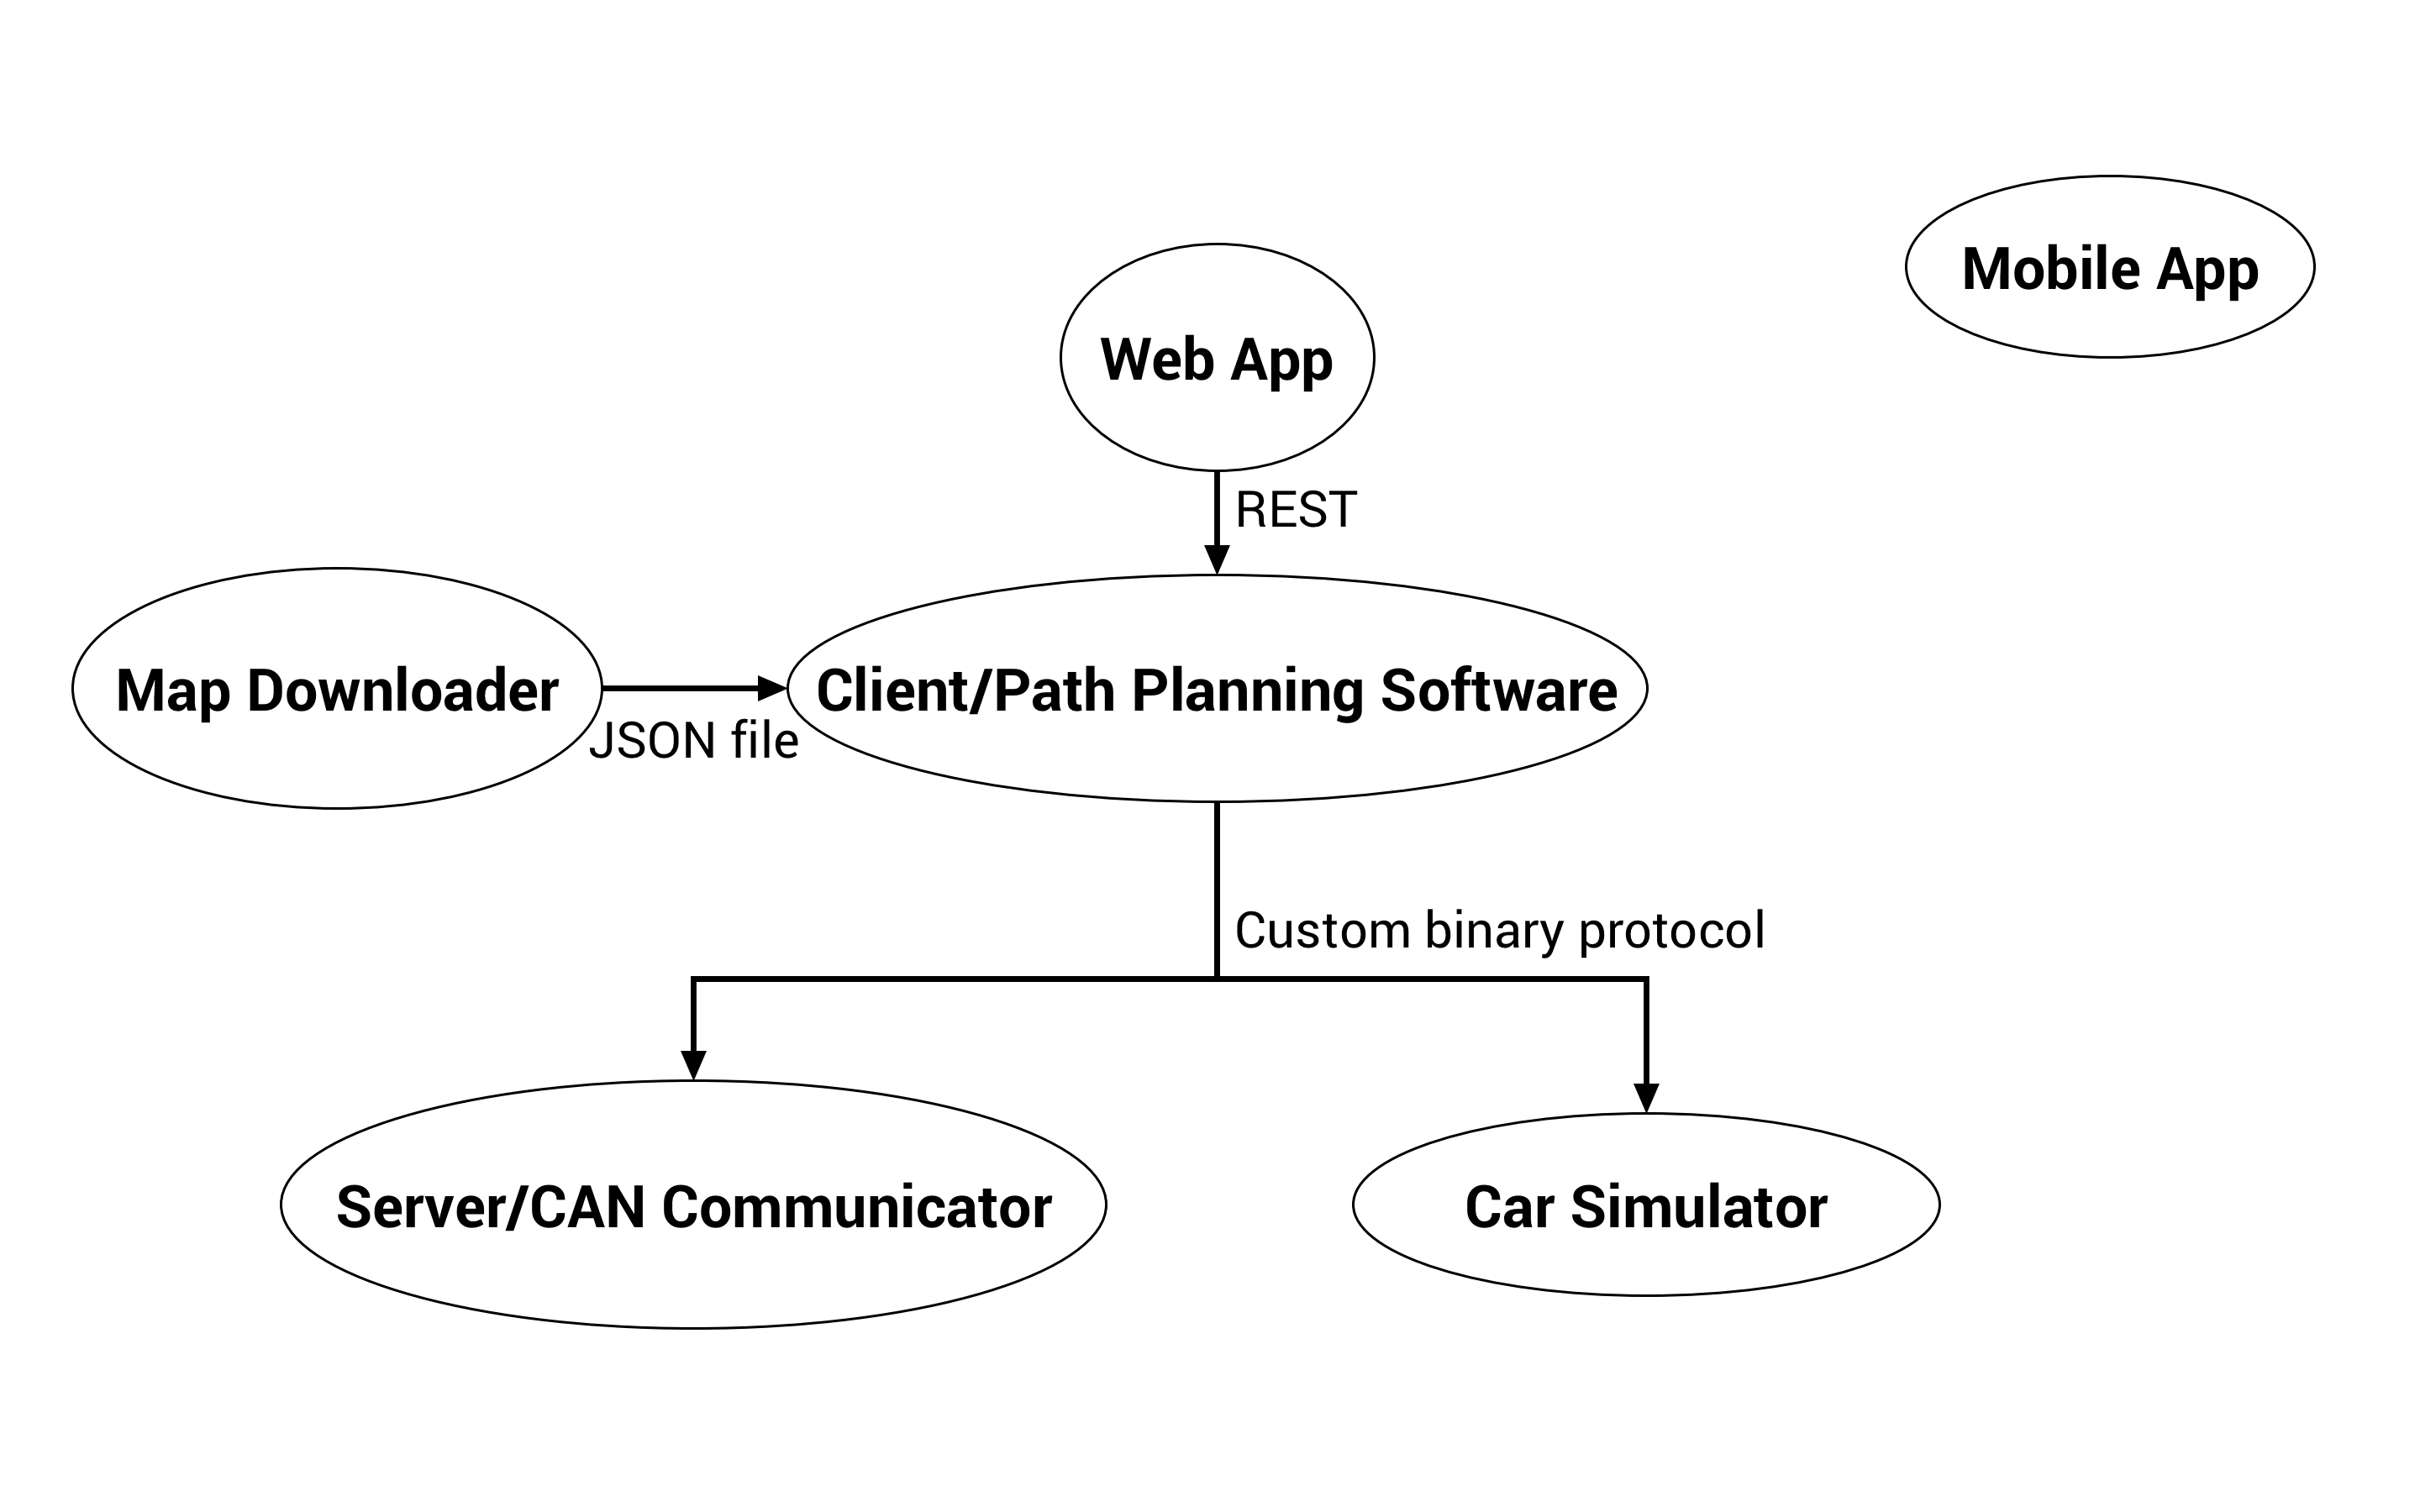
\includegraphics[width=0.9\columnwidth]{car-schema}
    \end{center}
\end{frame}

\begin{frame}
    \frametitle{Architektura projektu}
    \begin{center}
        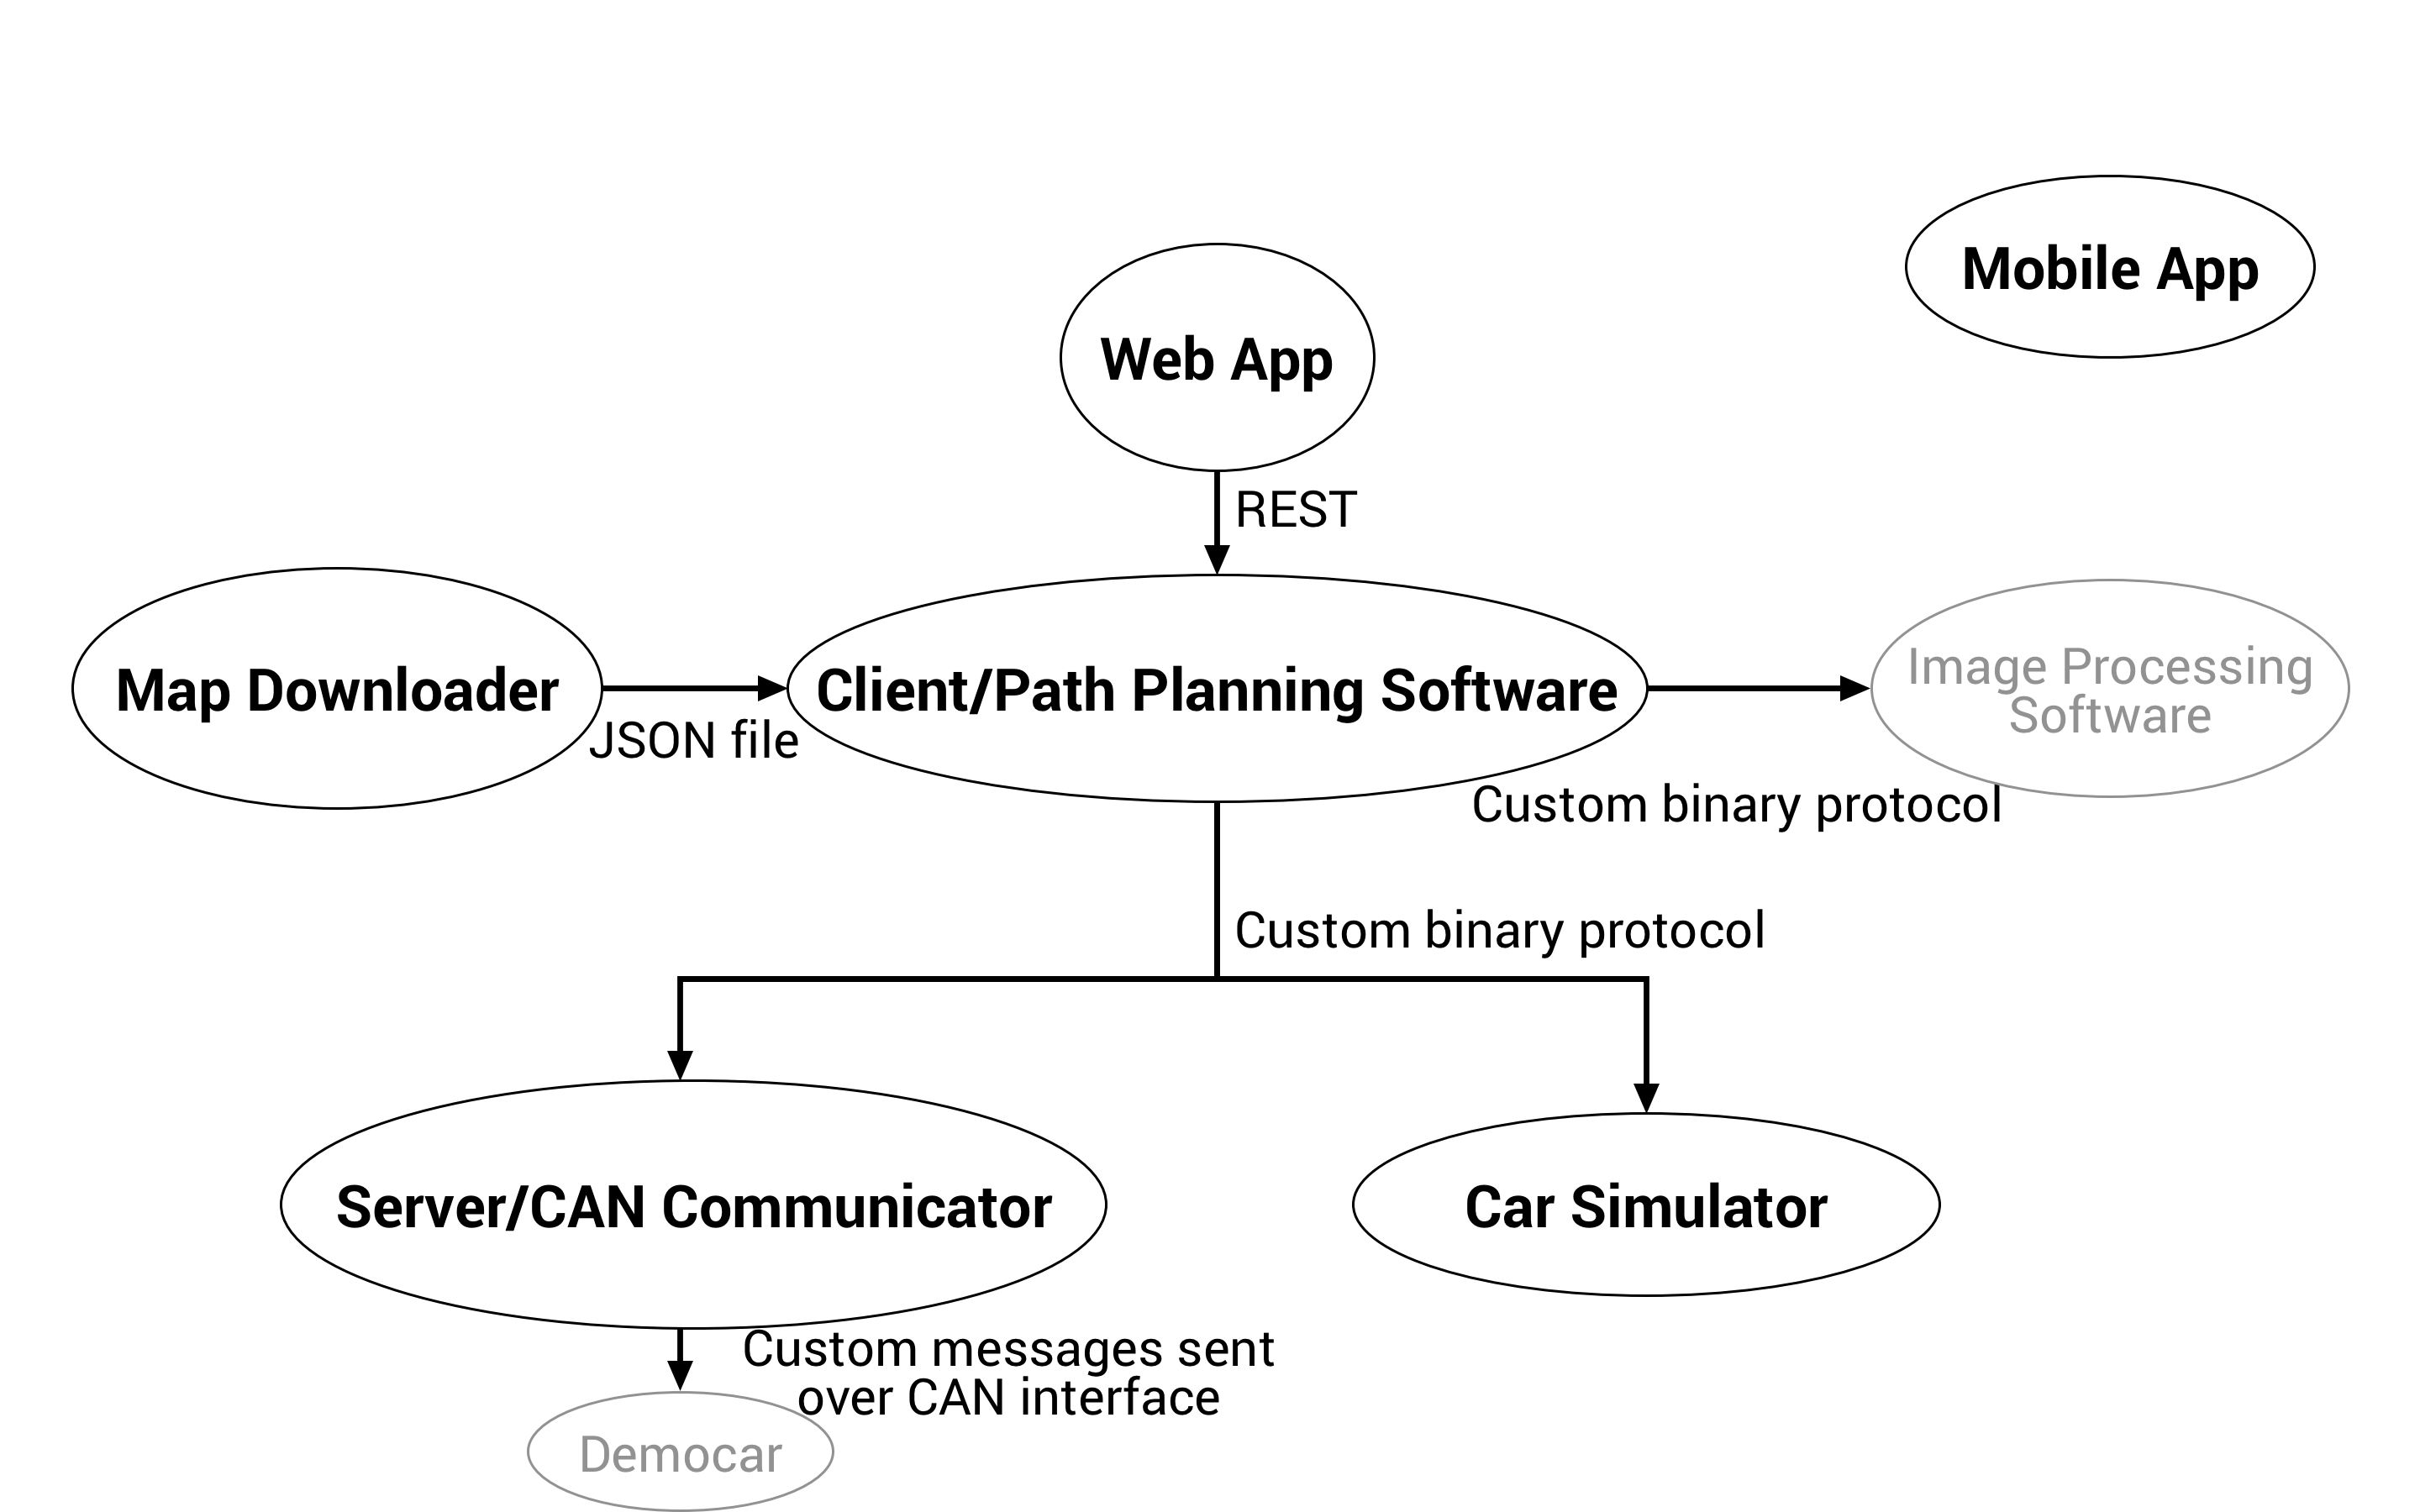
\includegraphics[width=0.9\columnwidth]{car-schema-full}
    \end{center}
\end{frame}

\section{Komponenty projektu}

\begin{frame}
    \frametitle{car-can}
    \begin{itemize}
        \item Python 3.8
        \item python-can
        \item Abstrakce komunikace přes CAN rozhraní
        \item Pomocí TCP rozhraní umožňuje předávat vozidlu pokyny
    \end{itemize}
\end{frame}

\begin{frame}
    \frametitle{car-simulator}
    \begin{itemize}
        \item Python 3.8
        \item Jednoduchá fyzika -- vozidlo je pouze hmotný bod
        \item Poskytuje stejné rozhraní jako CAN komunikátor
        \item Slouží především k jednoduchému testování
    \end{itemize}
\end{frame}

\begin{frame}
    \frametitle{car-client}
    \begin{itemize}
        \item Python 3.8
        \item Slouží k plánování cesty
        \item Komunikuje se serverem na vozidle
        \item Následování grafického bodu
        \item Následování GPS souřadnic
        \item Implementuje REST API umožňující zadání cíle cesty
        \item Práce s mapovými podklady
    \end{itemize}
\end{frame}

\begin{frame}
    \frametitle{car-webapp}
    \begin{itemize}
        \item Kotlin
        \item Mapy.cz
        \item REST API
        \item Webová aplikace
        \item Backend komunikuje s REST API plánovacího softwaru
        \item Backend validuje vstup -- veřejné API
        \item Umožňuje zadávat cíle cesty vozidla
        \item Umožňuje sledovat pozici vozidla
    \end{itemize}
\end{frame}

\begin{frame}
    \frametitle{car-map-downloader}
    \begin{itemize}
        \item Python 3.8
        \item Stahuje mapové podklady OSM
        \item Export dat do vlastního JSON formátu
        \item Lze naschedulovat cronem -- periodická obnova dat
    \end{itemize}
\end{frame}

\begin{frame}
    \frametitle{GeoLogger}
    \begin{itemize}
        \item Kotlin
        \item Jednoduchá Android aplikace
        \item Loguje GPS souřadnice do souboru
        \item Sloužila k testování přesnosti GPS
    \end{itemize}
\end{frame}

\section{Vývoj projektu a testování způsobů řízení}

\begin{frame}
    \frametitle{Vývoj projektu}
    \begin{itemize}
        \item Několik verzí CAN specifikace
        \item Několik způsobů řízení
            \begin{itemize}
                \item Řízení pomocí GPS
                \item Řízení pomocí detekce grafických kódů
                \item Řízení pomocí kombinace vstupů z kamer, GPS, LiDARu
            \end{itemize}
    \end{itemize}
\end{frame}

\begin{frame}
    \frametitle{Řízení pomocí GPS}
    \begin{itemize}
        \item Vozidlo jede rovne k nejbližšímu waypointu
        \item Řízeno pouze pomocí GPS
        \item Vysoká nepřesnost GPS
        \item Aplikace filtru pomohla, ale nedostatečně
    \end{itemize}
\end{frame}

\begin{frame}
    \frametitle{Řízení pomocí detekce grafických kódů}
    \begin{itemize}
        \item Pomocí kamery je detekován kód
        \item Plánovací software pozici kódu získá přes TCP rozhraní
        \item Vozidlo je vedeno přímo ke kódu
        \item Funkční, ale nepraktické
        \item Problém s fyzickým rozmístěním kódů
    \end{itemize}
\end{frame}

\begin{frame}
    \frametitle{Řízení pomocí vstupů z kamer, GPS, LiDARu}
    \begin{itemize}
        \item Vozidlo ledá cestu v mapových podkladech
        \item Danou cestu následuje
        \item Bezpečnost provozu, dodržování směru, atd. zajištěna kamerami
        \item Momentálně ve vývoji
    \end{itemize}
\end{frame}

\begin{frame}
    \frametitle{Dopad koronaviru}
    \begin{itemize}
        \item Znemožněno testování na fyzickém vozidle
        \item Nedostatek HW
        \item Plánovací software opožděn
        \item Čas byl využit k implementaci webové aplikace, obnově mapových podkladů
    \end{itemize}
\end{frame}

\section{Zhodnocení práce}

\begin{frame}
    \frametitle{Zhodnocení práce}
    \begin{itemize}
        \item Vyzkoušeny dva způsoby řízení
        \item Funkční komunikace přes rozhraní CAN
        \item Vzdálené ovládání vozidla pomocí TCP rozhraní
        \item Webová aplikace
        \item Základ řízení pomocí kombinace vstupů
        \item Vývoj bude pokračovat
    \end{itemize}
\end{frame}

\begin{frame}
    \frametitle{Konec}
    \begin{center}
        Děkuji za pozornost
    \end{center}
\end{frame}

\end{document}

